\documentclass{standalone}
\usepackage{tikz}
\usepackage{ctex,siunitx}
\setCJKmainfont{Noto Serif CJK SC}
\usepackage{tkz-euclide}
\usepackage{amsmath}
\usetikzlibrary{patterns, calc,3d}
\usetikzlibrary {decorations.pathmorphing,decorations.pathreplacing,decorations.shapes}
\begin{document}
\small
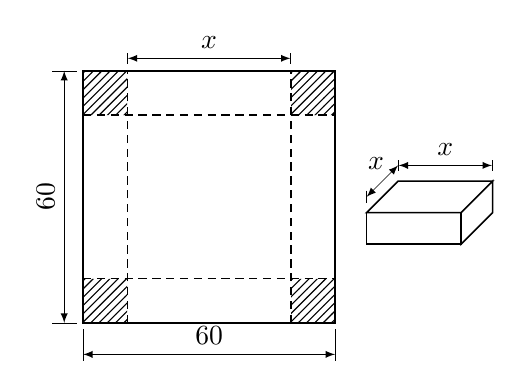
\begin{tikzpicture}[>=latex,scale=0.8]
  \fill[pattern=north east lines](2,-2)rectangle(1.3,-1.3)(-2,-2)rectangle(-1.3,-1.3)(2,2)rectangle(1.3,1.3)(-2,2)rectangle(-1.3,1.3);
  \draw[semithick](-2,-2)rectangle(2,2);
  \draw[densely dashed](-2,1.3)--(2,1.3)(-2,-1.3)--(2,-1.3)(1.3,-2)--(1.3,2)(-1.3,-2)--(-1.3,2);
  \draw[very thin,|<->|](-1.3,2.2)--(1.3,2.2)node[midway,above]{$x$};
  \draw[very thin,<->](-2,-2.5)--(2,-2.5)node[midway,above]{$60$};
  \draw[very thin,<->](-2.3,-2)--(-2.3,2)node[midway,sloped,above]{$60$};
  \draw[very thin](-2.1,2)--(-2.5,2)(-2.1,-2)--(-2.5,-2)(-2,-2.1)--(-2,-2.6)(2,-2.1)--(2,-2.6);
  \begin{scope}[xshift=3.5cm]
    \draw[semithick](-1,-0.25)--(0.5,-0.25)--(1,0.25)--(-0.5,0.25)--cycle(0.5,-0.75)--(0.5,-0.25)--(1,0.25)--(1,-0.25)--cycle;
    \draw[semithick](-1,-0.25)rectangle(0.5,-0.75);
    \draw[very thin,|<->|](-0.5,0.5)--(1,0.5)node[midway,above]{$x$};
    \draw[very thin,<->](-1,0)--(-0.5,0.5)node[pos=0.3,above=3pt]{$x$};
    \draw[very thin](-1,0.1)--(-1,-0.1);
  \end{scope}
\end{tikzpicture}
\end{document}